% This is samplepaper.tex, a sample chapter demonstrating the
% LLNCS macro package for Springer Computer Science proceedings;
% Version 2.20 of 2017/10/04
%
\documentclass[runningheads]{llncs}
%
\usepackage{graphicx}
\usepackage{url}
% Used for displaying a sample figure. If possible, figure files should
% be included in EPS format.
%
% If you use the hyperref package, please uncomment the following line
% to display URLs in blue roman font according to Springer's eBook style:
% \renewcommand\UrlFont{\color{blue}\rmfamily}

\begin{document}
%
\title{Visualizing High-dimensional Ball-Embeddings while Keeping Topological Relations\thanks{Supported by organization x.}}
%
%\titlerunning{Abbreviated paper title}
% If the paper title is too long for the running head, you can set
% an abbreviated paper title here
%
\author{First Author\inst{1} \and
Second Author\inst{1}  \and
Third Author\inst{1}  \and
Forth Author\inst{1}  \and
Fifth Author\inst{1,2}}
%
\authorrunning{F. Author et al.}
% First names are abbreviated in the running head.
% If there are more than two authors, 'et al.' is used.
%
\institute{University of Bonn, Germany  \\
\email{\{\}@uni-bonn.de}\\ 
\and
Fraunhofer IAIS, Germany\\
\email{}}
%
\maketitle              % typeset the header of the contribution

%150-250 words
\begin{abstract}
Region-based embeddings have been proven to be useful in knowledge graph reasoning. Existing visualization tool cannot preserve topological relations among high dimensional regions. We present a tool for visualizing high-dimensional balls that keeps topological relations after their dimensions are reduced to 2-dimensions. The first version of this tool provides four functions as follows: (1) Simple diagrammatic reasoning for syllogism; (2) diagrammatic reasoning with back-ground knowledge; (3) visualizing the construction process of ball-embeddings; (4) providing a web-service to impose a taxonomy structure onto its vector embeddings with zero-energy loss. A demonstration video of this tool is available at \dots. 
 
\keywords{Diagrammatic reasoning \and ball embeddings \and visualization.}
\end{abstract}
%
%
%
\section{Introduction}

 Bing able to learn from data, and robust to noisy inputs, Deep-Learning has been successful in a variety of AI tasks that have frustrated classic symbolic approaches for decades, such as object classification, machine translation, voice recognition, question-answering \cite{LeCunNature15}. However, Deep-Learning  Systems lack of explainability, can be fooled \cite{BiDAF16,JiaLiangaL17,Belinkov17}, and normally need much more learning data than human does \cite{tenenbaum15}. This introduces potential dangers into safety critical applications, such as autonomous driving. Introducing innate structures into Deep-Learning system has been advocated, and listed as one of the AI research topics in the Townhall meeting at AAAI-19, so that Deep-Learning research shall solve logical reasoning tasks (System 2 of mind) \cite{Kahneman11,benjio19}. As logical reasoning, such as Syllogism, is better represented by inclusion relations among regions, instead of translation among vectors \cite{Venn1880,diagram95}, recent researches have been attempting to promote vectors into regions to improve performances of logical query, triple classification, link prediction of Knowledge Graph \cite{dong19iclr,dong19,li2019smoothing,JuanziEmnlp18,ren2020}.   

% Though a powerful tool for learning from data, Deep Learning limits itself in representing everything as vectors, and can only approximate symbolic representation and reasoning. This limitation can be approached by promoting vector embeddings to ball embeddings. Vector embeddings of nodes in a taxonomy structure can be promoted into balls in higher-dimensional space, such that (1) each vector embedding is well preserved by the central point of a ball; (2) child-parent relations are precisely encoded by inclusion relations among balls. Significant results are obtained in experiments on unifying word-embeddings with hypernym trees and on unifying entity-embeddings learned from knowledge-graphs and tree structures. Being able to precisely imposing external symbolic structures onto Deep Learning systems not only paves the way towards resolving the antagonism between connectionism and symbolicism in the literature, but also has tremendous value in real applications. For example, being able to impose traffic rules onto autonomous driving cars would ultimately solve the safety issue.  

% Taxonomy, as a classification of concepts, exists in almost every disciplinary, such as file systems in computer science , government organization of a country, classification of viruses, plants, and animals. 

% Ball embeddings are rigorously constructed by a sequence of geometric transformations under the  condition that the loss function of the embedding must be zero, which is a condition that is not required and has not been targeted by Deep Learning approaches. This also raises the visualization problem of ball embeddings. 
The popular  tool t-NSE \cite{Maaten08} for visualizing vector embeddings cannot be directly applied for visualizing ball embeddings, for the dimensional reduction process of t-NSE does not guarantee the topological relations among balls. In this paper, we demonstrate an open source system that is able to visualize ball embeddings while keeping their topological relations. The main contributions of this system are as follows: (1) it has an vivid interactive user interface that can be used for diagrammatic reasoning among taxonomy; (2) it provides an effective and friendly approach for debugging the geometric construction process of ball embeddings; (3) it provides a batch service that accepts a large scale input for construct ball embeddings. 

\section{The Architecture}

In order to provide useful visual feedback for the construction process of the ball embeddings the user needs to provide a history of the construction of their ball embeddings. In order to make the system more accessible and allow for quick demonstrations purposes we allow the user to alternatively provide a set of words along with their taxonomy. Using the approach of [] we then compute a set of high quality word embedding along with their construction history.

To make the system accessible from almost any modern devise we chose to expose the user interface through a website. The user request is accepted by a flask web-server and placed in compute queue to allow for concurrent access and real-time feedback for the user even if the server is busy. 

Finally given the ball embedding history we determine for every step if any two N-balls intersect, contain each other or are separate. This allows us to create a visual feedback reminiscent of a debugger of the N-balls construction along with a input taxonomy as a tree. Not only can the user see when his approach violates the taxonomy but also how and with which participant.

\begin{figure}
\center
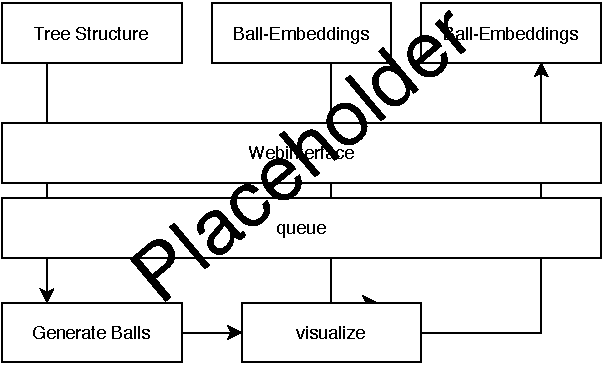
\includegraphics[width=0.85\textwidth]{res/diagram-crop}
\caption{Some caption}
\label{fig::architecture}
\end{figure}


\section{Services}

\subsection{Simple Diagrammatic Reasoning}

Ball embeddings allow for strict reasoning and logical queries. This can be demonstrated with our tool. The user can input hypernym relationships in plain English such as "socrates is human, human is animal" we display that relationship as seen in figure X. Similarity system also handles exclusion such as "soccer is not human,human is mortal" as seen in figure X. Once these relations have been enforced on the sufficiently large corpus, ideally for all words present in the underlying word embedding, this allows for strict logic varies which are otherwise impossible in neural networks.
 
\subsection{Diagrammatic Reasoning with Background Knowledge} 
\begin{itemize}
	\item user input: Soccer is not human, human is animal
	\item  user query: what is the relation between Soccer and animal
	\item  system replaces `Soccer is not human' with `Soccer is entity', system adds 'animal is entity' by searching background knowledge
	\begin{verbatim}
		>>> from nltk.corpus import wordnet as wn
>>> soccer = wn.synsets('soccer')
>>> soccer
[Synset('soccer.n.01')]
>>> soccer = wn.synsets('soccer')[0]
>>> soccer
Synset('soccer.n.01')
>>> human=wn.synsets('human')[0]
>>> human
Synset('homo.n.02') 
>>> soccer.lowest_common_hypernyms(human)
[Synset('entity.n.01')] 
>> % check 'animal' and 'entity'
>> ..
	\end{verbatim}
\item  system draw: (1) Soccer ball outside animal ball, (2) human ball inside animal ball; (3) they are inside entity ball 
	\item system merges (1), (2), and (3)  
	\item system conclude: Soccer is not animal.
\end{itemize}

\subsection{Visual Debugging}
Enforcing a relational structure onto word embedding is a difficult task. Similar to a code-debugger we provide a visual feedback for every construction step which; (1) allows the viewer to retrace and understand the construction process and as such serves as a valuable teaching tool; (2) enables developers to optimize {and correct their ball embedding construction.

Since we only consider hierarchical structures in this paper we can guarantee that any valid state can be visualized on to a two dimensional canvas. In order to achieve this we first construct a set of nonoverlapping circles that perfectly represents the hierarchy that is to be encoded into the ball embeddings. Then within each construction step we either display the previously computed perfect representation or enforce any overlapping's that have been recorded in the ball embedding construction history.

\subsection{Batch Service}

\begin{itemize}
	\item user provide her/his name and contact email.
	\item user input: a tree structure, vector embeddings of tree nodes
	\item System will construct ball embeddings at backend, and send the user the link fo the final ball embeddings  
\end{itemize}

\section{Conclusion and Outlooks}

link to the video

 
%
% ---- Bibliography ----
%
% BibTeX users should specify bibliography style 'splncs04'.
% References will then be sorted and formatted in the correct style.
%
% \bibliographystyle{splncs04}
% \bibliography{mybibliography}

\bibliographystyle{plain}
\bibliography{XBib_NN,XBib} 
\end{document}
